\chapter{Opis zajedničke AST apstrakcije}
\label{chp:MyAST}

Kako bi se kreirala smislena apstrakcija stabla parsiranja, potrebno je identifikovati bitnih informacije u stablu parsiranja ali i koncepte same gramatike koji su od značaja. Najjednostavnije rešenje je mimikovati čvorove stabla parsiranja, ukoliko su gramatička pravila kreirana tako da oslikaju koncepte jezika koji gramatika definiše. Na primer, ukoliko u gramatici imamo pravilo \texttt{deklaracija} sa alternativama \texttt{deklaracijaPromenljive} i \texttt{deklaracijaFunkcije}, možemo apstrakciju posmatrati kao apstraktnu klasu \texttt{Deklaracija} sa konkretizacijama \texttt{DeklaracijaPromenljive} i \texttt{DeklaracijaFunkcije}. Kako se definišu deklaracije promenljivih i funkcija zavisi dalje od definicija pravila \texttt{deklaracijaPromenljive} i \texttt{deklaracijaFunkcije}. Naravno, nije uvek moguće primeniti ovakav postupak. Takođe, nekada u gramatici definišemo pomoćna pravila kako bismo se izborili sa rekurzijom ili izbegli neke tipove rekurzije - ta pravila ne bi trebalo da imaju odgovarajuće tipove u apstrakciji. Dakle, identifikovanje toga šta čini gramatiku nije jednostavno u opštem slučaju. Međutim, pošto su u pitanju gramatike programskih jezika, onda je jasno da dosta različitih gramatika dele slične koncepte i da je moguće definisati tipove čvorova koji odgovaraju tim konceptima. Neki od njih mogu biti: naredba, izraz, deklaracija, poziv funkcije, dodela... Jasno, postoji i hijerarhija u navedenom - recimo poziv funkcije se može smatrati kao samostalna naredba ali može biti i deo izraza. Dakle, treba biti jako pažljiv u definisanju hijerarhije tako da ne dozvoli nešto što u opštem slučaju ne bi trebalo da bude dozvoljeno (npr. ako je dozvoljeno višestruko nasleđivanje i poziv funkcije je i naredba ali i izraz, onda se izrazi u kojima figurišu pozivi funkcija sastoje od više naredbi, što nema smisla.).

Bez obzira na to koje koncepte izdvojimo iz stabla parsiranja kao relevantne, potrebno ih je sve unifikovati. Slično kao što svi čvorovi stabla parsiranja moraju biti derivati određene klase (pošto svi elementi stabla moraju biti istog tipa), isto treba da važi i za apstraktno sintaksno stablo. Stoga, postojaće apstraktna bazna klasa sa informacijama koje svaki čvor AST-a poseduje. Ova bazna klasa će u nastavku rada biti referisana kao \texttt{ASTNode}. Pošto je AST stablo u kome svaki čvor može imati proizvoljno mnogo potomaka, očekivano je da svaki čvor ima pokazivače na potomke gde svaki pokazivač pokazuje na objekat tipa \texttt{ASTNode} (jasno, ne možemo napraviti objekat klase \texttt{ASTNode} jer je klasa apstraktna ali konkretizacije klase \texttt{ASTNode} su takođe tipa \texttt{ASTNode}). Radi jednostavnosti implementacije nekih operacija biće dodatno dostupna informacija o roditelju svakog čvora putem pokazivača na roditelja, tipa \texttt{ASTNode} - koreni čvor neće imati postavljenu vrednost ovog polja. Dodatne informacije recimo mogu biti linija u izvornom fajlu gde se nalazi kod koji odgovara čvoru. Dodatno, možemo definisati i metode koje treba svaki čvor da poseduje - recimo metode za serijalizaciju \footnote{Serijalizacija predstavlja proces konvertovanja stanja objekta u niz bajtova da bi se isti sačuvao u bazu podataka, fajl, ili pak prosledio nekom drugom programu.}. 

\begin{figure}[h!]
    \centering
        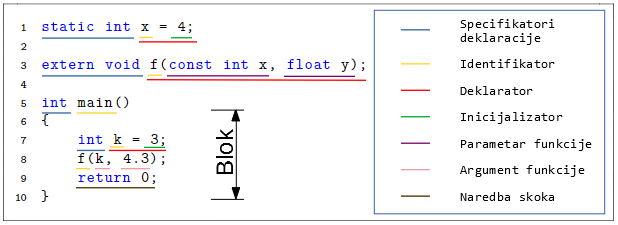
\includegraphics[scale=0.9]{images/c_code_decomposition.png}
    \caption{Vizualni prikaz delova C koda na osnovu pravila iz C11 gramatike.}
    \label{fig:CDecomposition}
\end{figure}

Krenućemo od gramatika strogo tipiziranih proceduralnih programskih jezika, a zatim ćemo koncepte proširiti i na skript jezie. U strogo tipiziranim proceduralnim jezicima se mogu identifikovati koncepti koji se pojavljuju u većini od njih. Na primeru C koda sa slike \ref{fig:CDecomposition} moguće je videti neke od njih. Koncepti naredbe i izraza su očigledni i nisu prikazani. Nije očigledno, doduše, kako bi se deklaracija promenljive dekomponovala na delove. Po C11 gramatici, svaka deklaracija se sastoji od \emph{specifikatora deklaracije} i od jednog ili više \emph{deklaratora}. Specifikatori deklaracije su ključne reči koje bliže određuju deklaraciju - modifikatori vidljivosti ili specifikatori pristupa. Deklaratori uvode simbol (\emph{identifikator}) u kontekst kao promenljivu, niz ili funkciju. Deklaratori, u zavisnosti od toga šta se deklariše, mogu imati razne delove. Ukoliko je u pitanju deklarator promenljive, sastoje se i od opcionog izraza za inicijalizaciju, u daljem tekstu \emph{inicijalizator}. Ukoliko je u pitanju deklarator funkcije, nakon identifikatora se nalazi lista parametara funkcije - svaki od njih se sastoji od specifikatora deklaracije i deklaratora.

Ovakvi koncepti će biti inspiracija za definisanje AST čvorova, pri čemu će detaljno biti opisana motivacija i razlozi za odabir nekih specifičnosti. Koren svakog AST-a će biti tipa \texttt{TranslationUnitNode} - direktne konkretizacije klase \texttt{ASTNode}, bez dodatnih polja i metoda. Jedina svrha ove klase je da označi granice izvornih fajlova u slučaju da se pravi AST od više različitih izvornih fajlova. U nastavku će biti opisane složenije konkretizacije klase \texttt{ASTNode} grupisane po nameni. 

